% !TeX root = ../main.tex

\subsection{3D 列印部件}
為了完整記錄本系統的所有客製化組件，本節依據 3D CAD 裝配模型，將系統中使用的主要 3D 列印部件分類並條列說明如下。

\subsubsection{光學部分}

明視野 LED 座 (Brightfield\_LED\_Mount)：用於安裝系統頂部的白光 LED 光源。考量到 LED 長時間運作的發熱問題，此固定座特別加大與空氣接觸的表面積以利散熱，並具備防呆定位槽，確保 LED 發光中心精確對準聚光鏡的入瞳。此外，當此底座與聚光鏡座組合時，LED 發光面恰好位於聚光鏡的焦平面上，藉此達成最佳位置配置。


\begin{figure}[H]
    \centering
    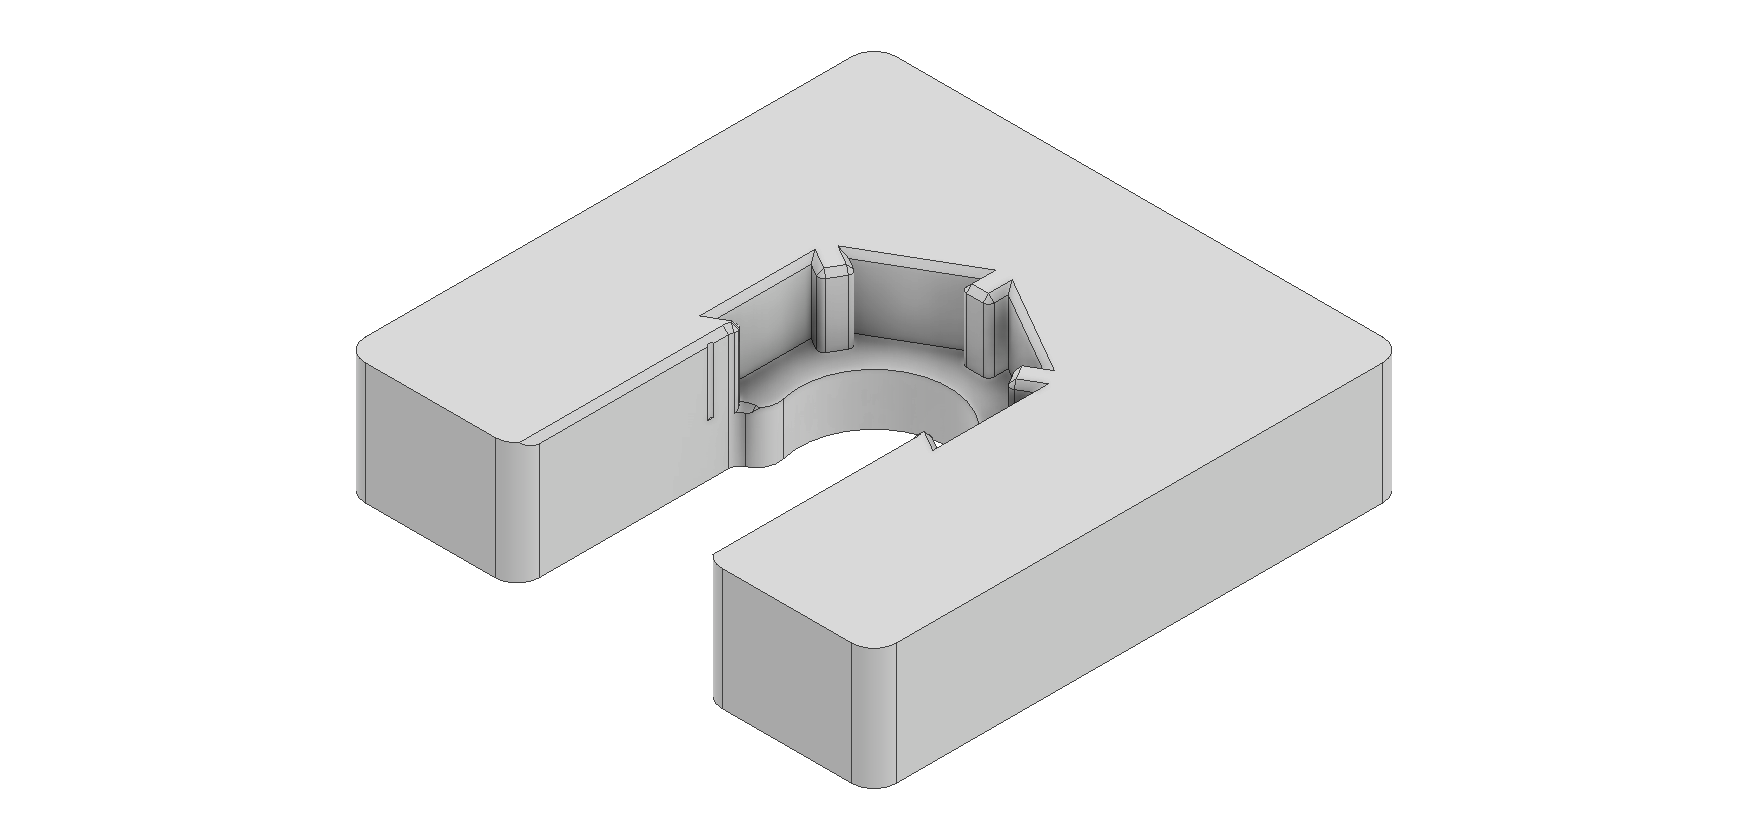
\includegraphics[width=\textwidth]{figures/ch3/fig3_11_Brightfield_LED_Mount.png}
    \caption{明視野 LED 座 (Brightfield\_LED\_Mount)}
    \label{fig:part_brightfield_led_mount}
\end{figure}

明視野聚光鏡座 (Brightfield\_Condenser\_Mount)：此部件專為明視野照明系統中的非球面聚光鏡所設計。其內部具備上大下小的三角形定位面，透過施加壓力與摩擦力實現三點固定法，能精確夾持聚光鏡，並透過底部的樂高插銷結構與剛性框架卡合，確保聚光鏡與下方物鏡的成像光軸達成微米級的共軸對齊，從而提供均勻且高數值孔徑（NA）的穿透式照明。
\begin{figure}[H]
    \centering
    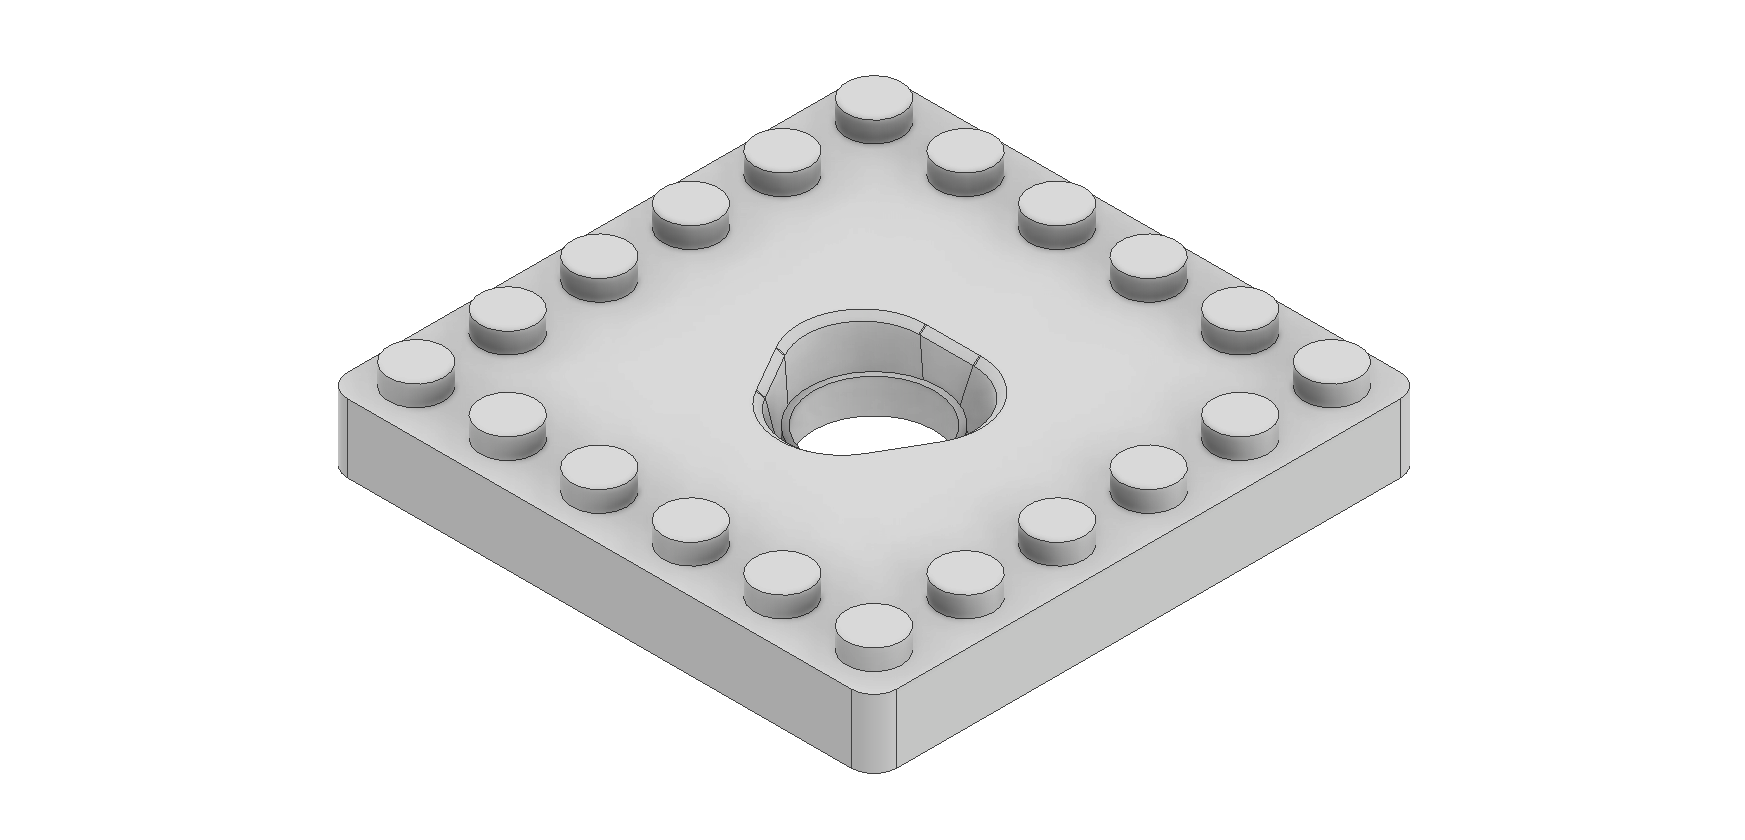
\includegraphics[width=\textwidth]{figures/ch3/fig3_12_Brightfield_Condenser_Mount.png}
    \caption{明視野聚光鏡座 (Brightfield\_Condenser\_Mount)}
    \label{fig:part_brightfield_condenser_mount}
\end{figure}

物鏡轉接座 (Objective\_Mount)：為本系統連接顯微物鏡與樂高剛性框架的關鍵核心轉接件。此部件內部設計有符合國際標準的 RMS（Royal Microscopical Society）螺紋，能直接鎖入標準顯微物鏡，其下側則具備與樂高卡合的結構以確保光軸的同軸性，而非提供高剛性與定位重複性。透過此標準化的螺紋介面，使用者能輕易替換不同放大倍率的物鏡，快速切換觀察模式。
\begin{figure}[H]
    \centering
    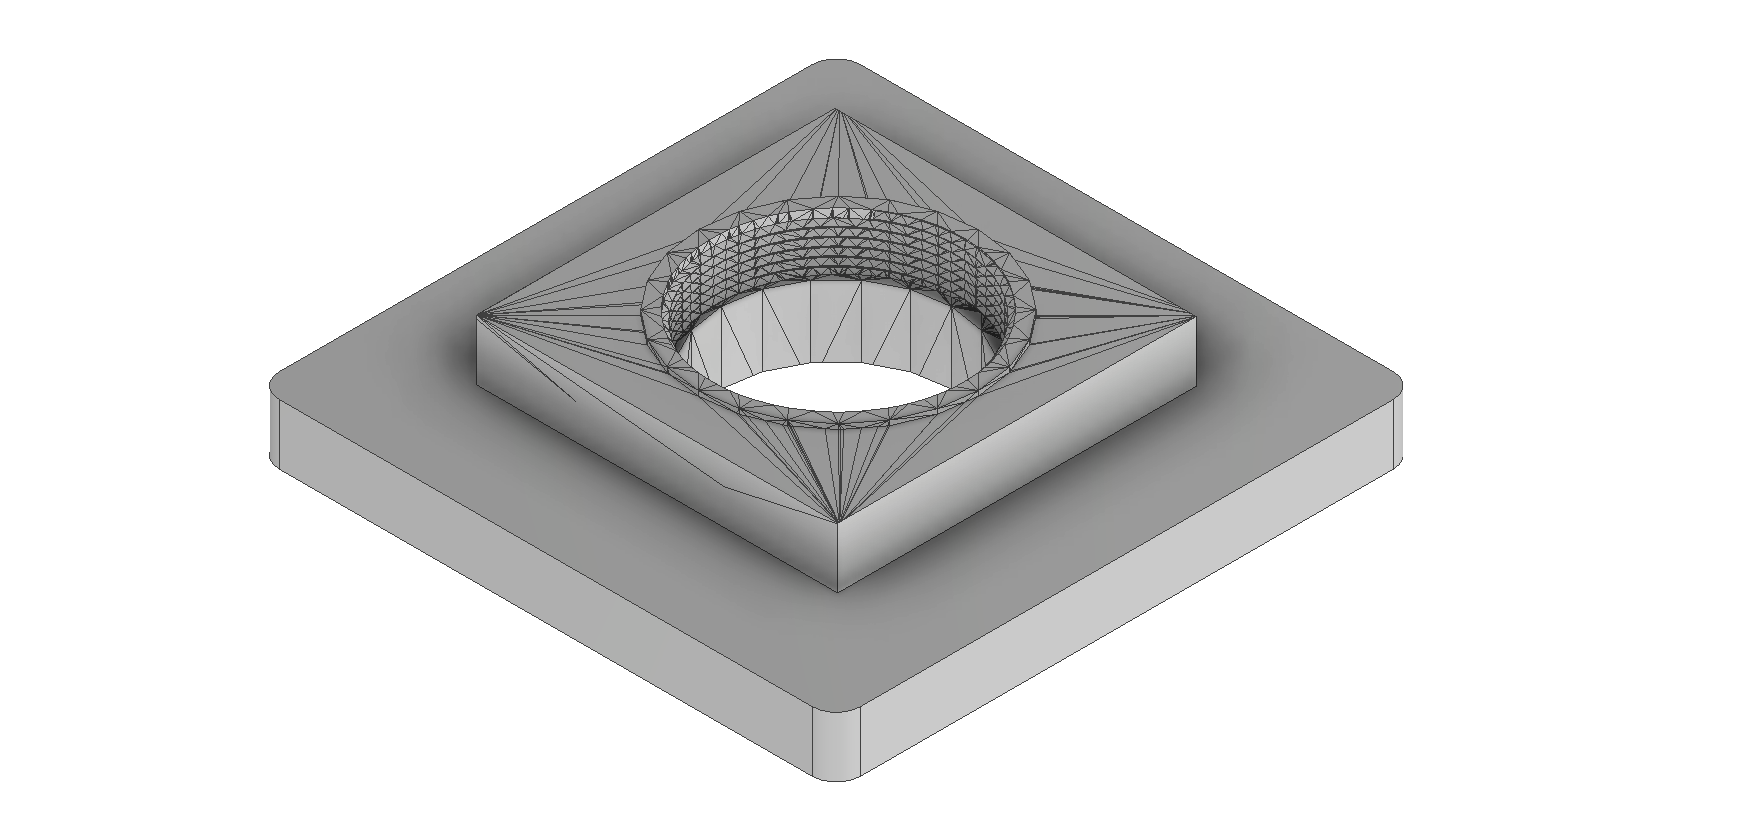
\includegraphics[width=\textwidth]{figures/ch3/fig3_13_Objective_Mount.png}
    \caption{物鏡轉接座 (Objective\_Mount)}
    \label{fig:part_objective_mount}
\end{figure}

濾光方塊座 (Filter\_Cube\_Mount)：為本系統螢光成像模組的核心樞紐。其內部空間經過嚴密幾何設計，以標準 $45^\circ$ 角固定雙色分光鏡（Dichroic Mirror），並在正交方向上預留激發與發射光路通道；其下半部並預留有放置發射濾光片（Emission Filter）的空間，使濾光方塊整合了雙色分光鏡與發射濾光片兩項功能。此部件底部同樣具備樂高相容結構，是實現落射式螢光激發與採集分離的關鍵機構。
\begin{figure}[H]
    \centering
    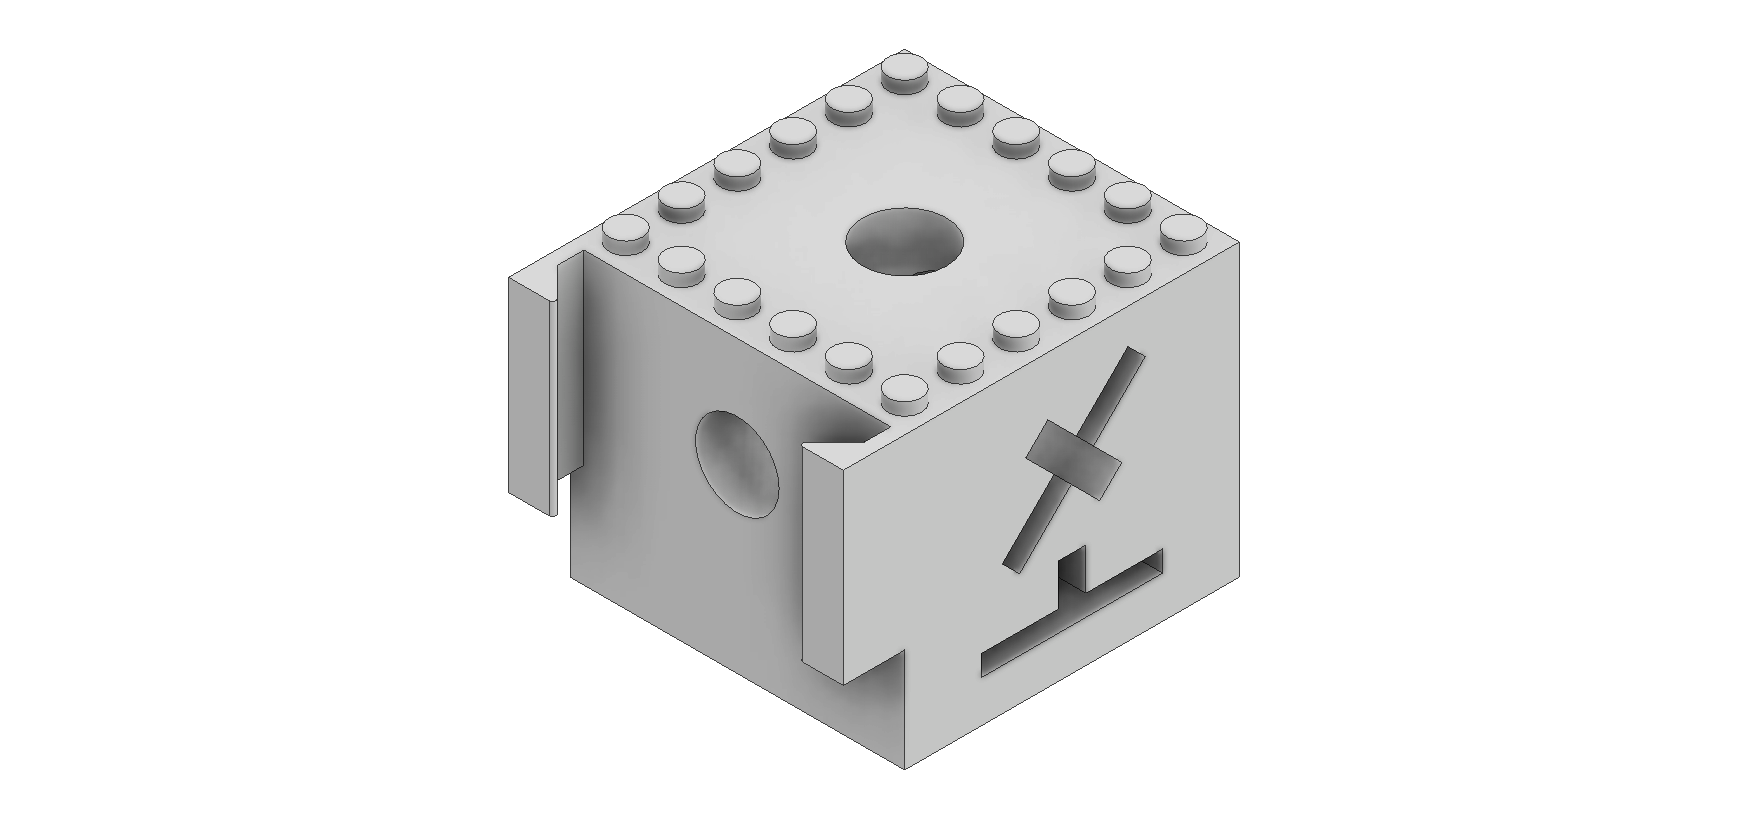
\includegraphics[width=\textwidth]{figures/ch3/fig3_14_Filter_Cube_Mount.png}
    \caption{濾光方塊座 (Filter\_Cube\_Mount)}
    \label{fig:part_filter_cube_mount}
\end{figure}

激發濾光片座 (Excitation\_Filter\_Mount)：用於在激發光路中精確固定短通（Shortpass）激發濾光片。其設計與擴散片座相呼應，同樣具備便於快速抽換的鑷子夾取孔位，以及確保濾光片重力自擺正的圓弧滑軌，讓使用者在不必拆卸周邊元件的情況下即可快速更換濾光片，大幅提升了多色螢光實驗的便利性。
\begin{figure}[H]
    \centering
    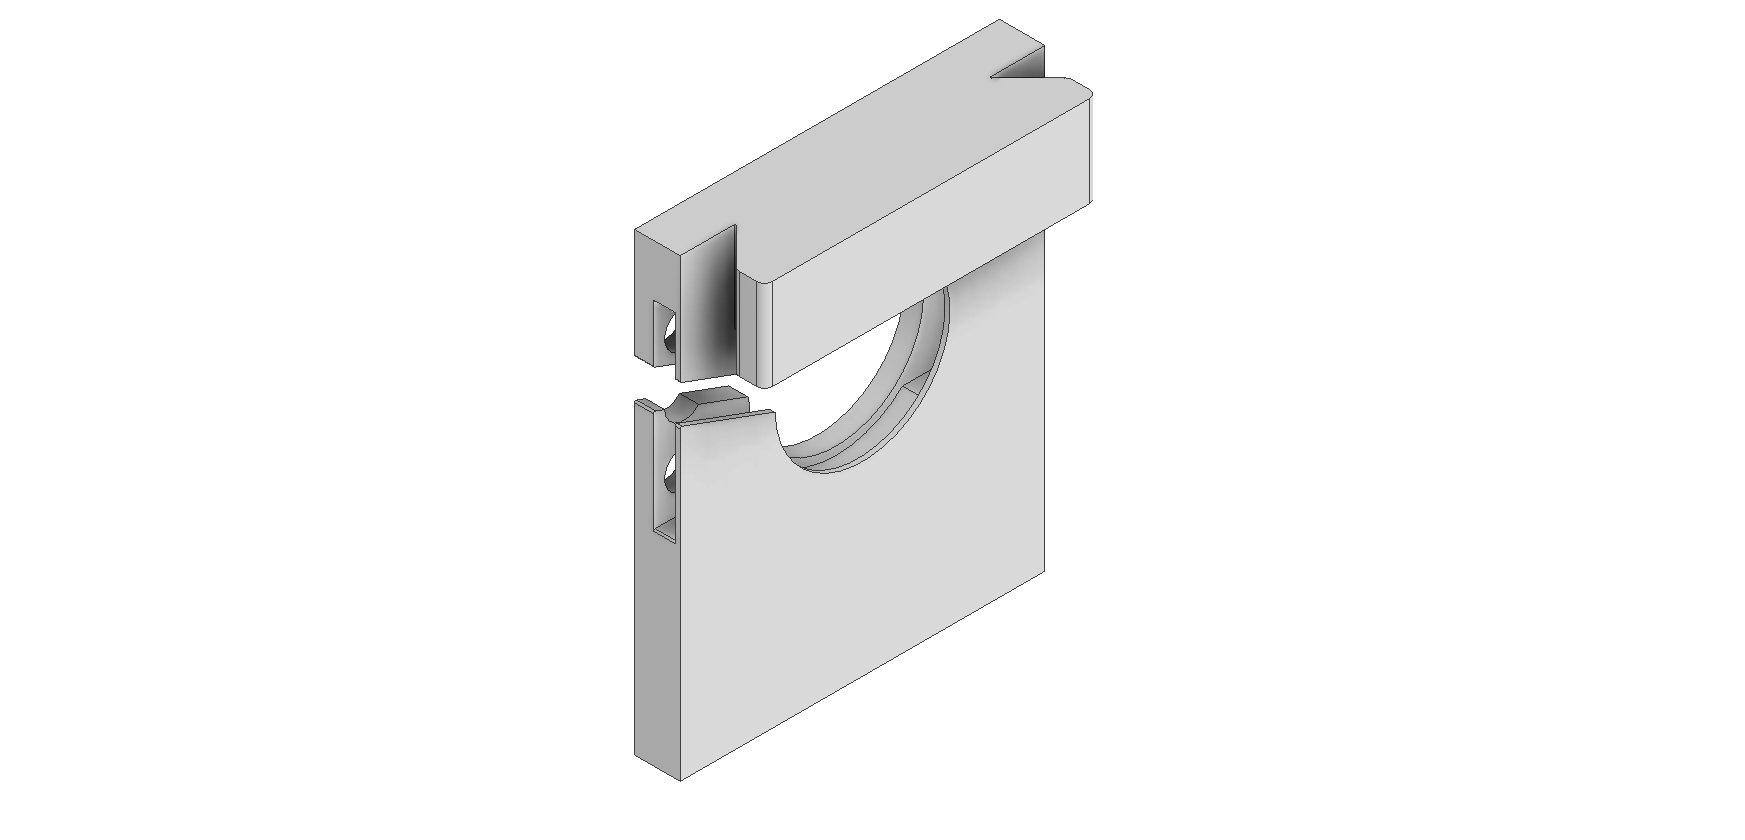
\includegraphics[width=\textwidth]{figures/ch3/fig3_15_Excitation_Filter_Mount.png}
    \caption{激發濾光片座 (Excitation\_Filter\_Mount)}
    \label{fig:part_excitation_filter_mount}
\end{figure}

螢光聚光鏡座 (Fluorescence\_Condenser\_Mount)：專用於螢光激發光路中固定非球面聚光鏡。此部件內部同樣具備上大下小的三角形定位面，透過施加壓力與摩擦力實現三點固定法，能精確夾持聚光鏡，並透過底部的樂高插銷結構與剛性框架卡合，確保聚光鏡與激發光軸達成高精度的同軸對齊。
\begin{figure}[H]
    \centering
    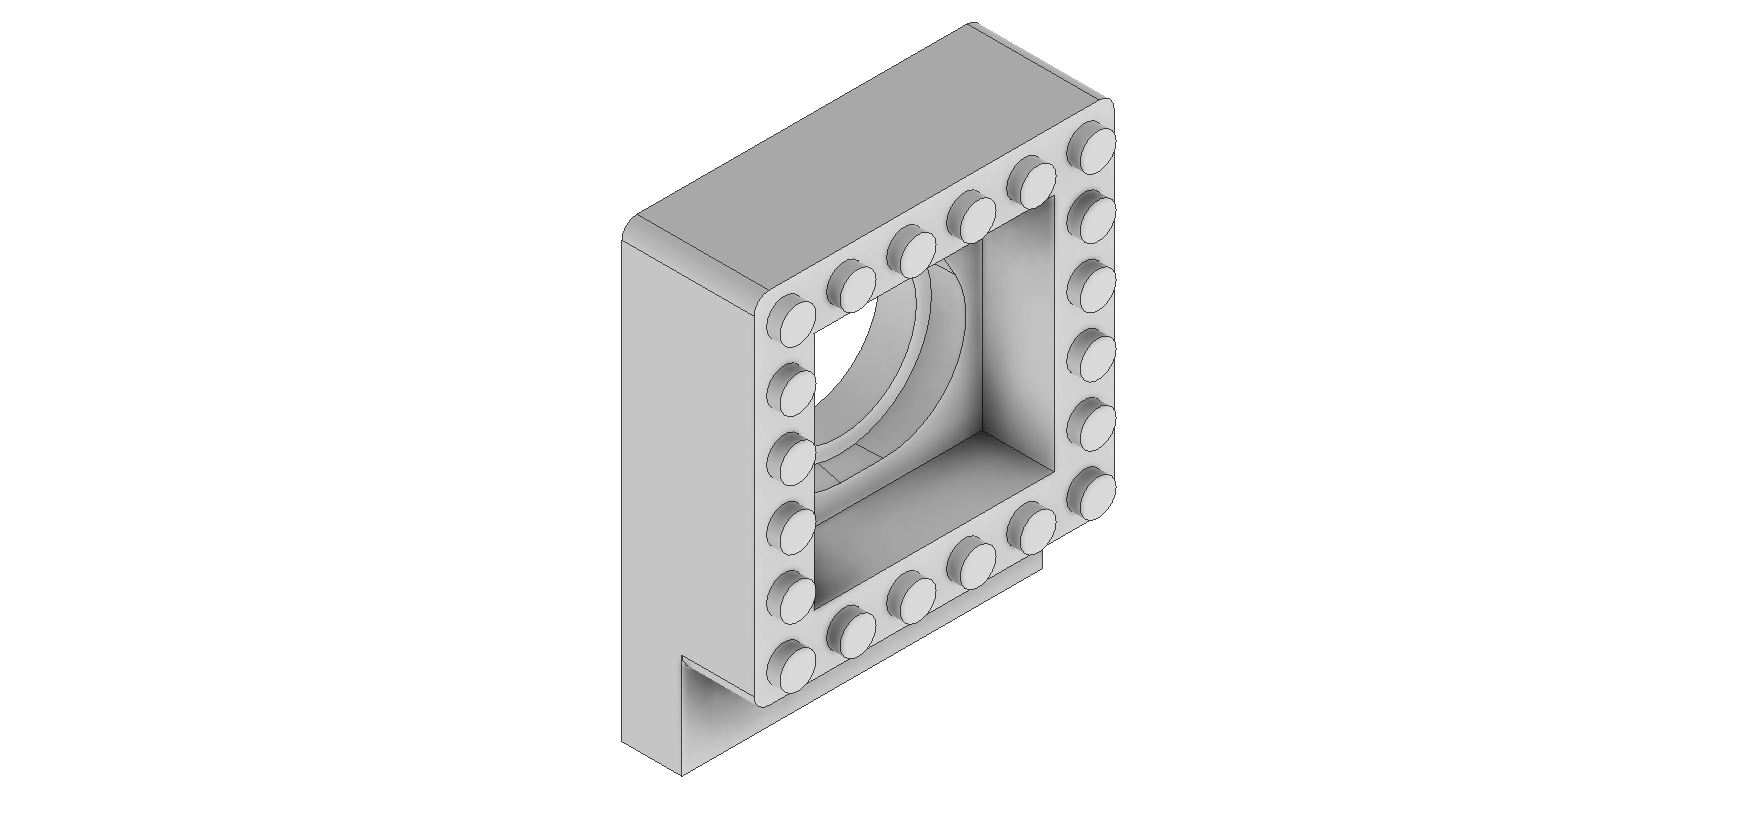
\includegraphics[width=\textwidth]{figures/ch3/fig3_16_Fluorescence_Condenser_Mount.png}
    \caption{螢光聚光鏡座 (Fluorescence\_Condenser\_Mount)}
    \label{fig:part_fluorescence_condenser_mount}
\end{figure}

螢光 LED 座 (Fluorescence\_LED\_Mount)：用於搭載激發螢光所需的高功率藍光 LED。由於高功率運作時會產生顯著熱量，此固定座結構上特別設計了大型導熱接觸面，以加大與空氣接觸的散熱面積，維持 LED 的發光效率與壽命。
\begin{figure}[H]
    \centering
    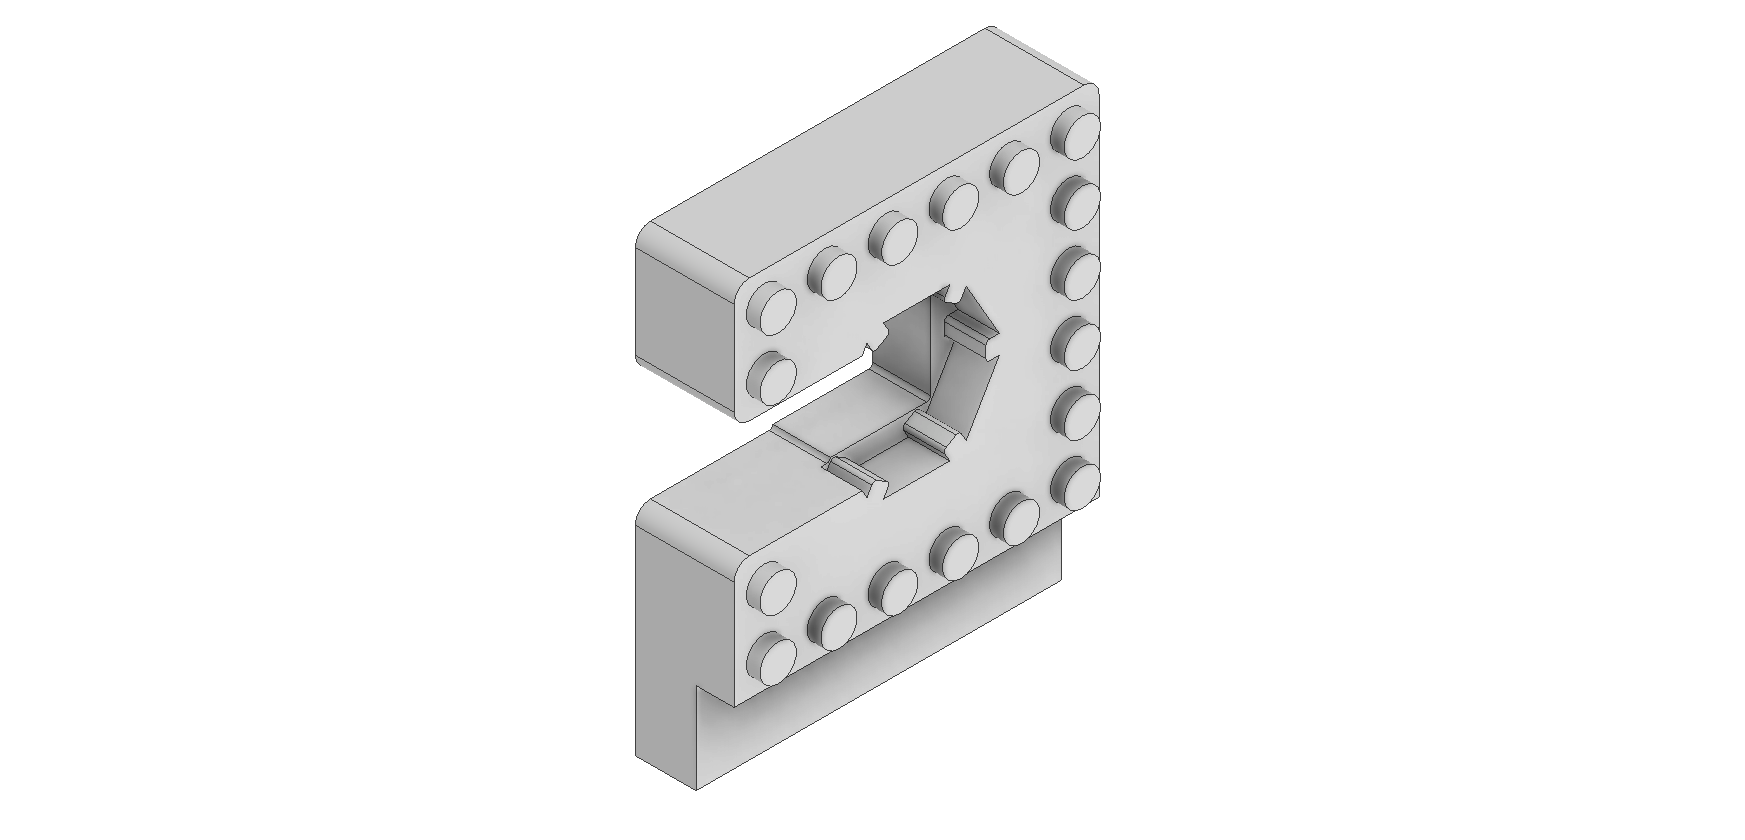
\includegraphics[width=\textwidth]{figures/ch3/fig3_17_Fluorescence_LED_Mount.png}
    \caption{螢光 LED 座 (Fluorescence\_LED\_Mount)}
    \label{fig:part_fluorescence_led_mount}
\end{figure}

螢光雷射座 (Fluorescence\_Laser\_Mount)：為雷射激發光源提供穩固的剛性支撐。雷射模組本體為圓形，外接一個正方形柱體以加大散熱面積，因此此座體內框設計為正方形，以緊密包覆雷射模組的正方形外殼；頂部並設有螺絲與螺帽，透過頂抵外框的方式實現牢固的徑向固定，避免掃描運動時的微小震動導致激發光斑發生漂移。
\begin{figure}[H]
    \centering
    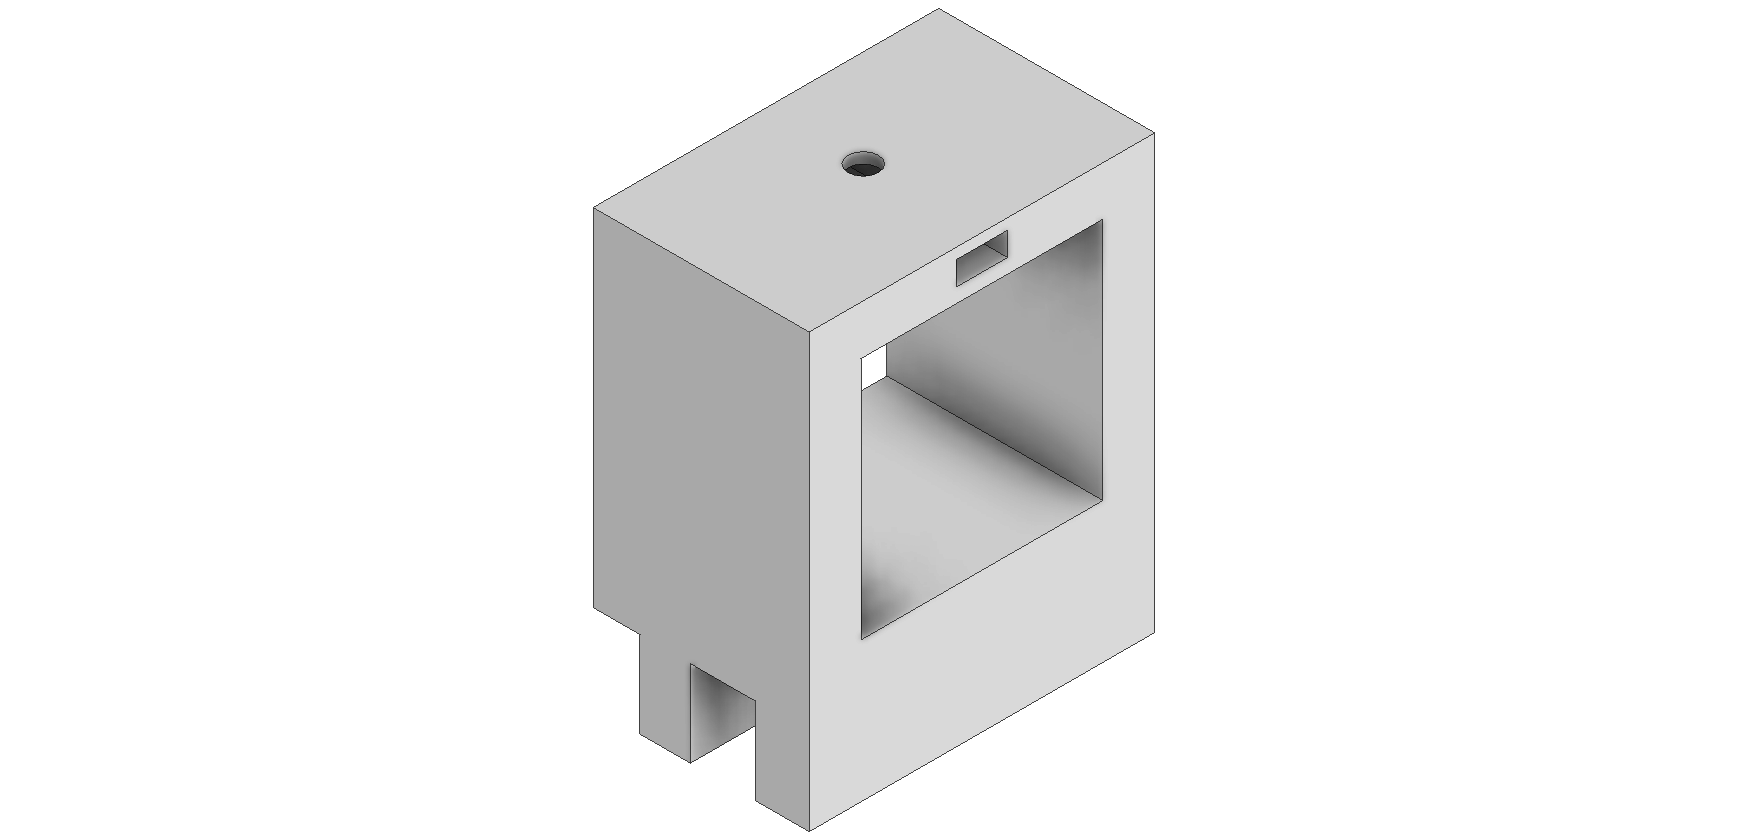
\includegraphics[width=\textwidth]{figures/ch3/fig3_18_Fluorescence_Laser_Mount.png}
    \caption{螢光雷射座 (Fluorescence\_Laser\_Mount)}
    \label{fig:part_fluorescence_laser_mount}
\end{figure}

擴散片座 (Diffuser\_Mount)：用於在螢光激發光路中固定光學擴散片，以均勻化雷射或 LED 的光斑。此部件特別融入了人性化設計，頂部設有方便鑷子夾取的長方形凹槽，內部則有利用重力原理的圓弧導引槽，讓使用者在不必拆卸周邊元件的情況下即可快速更換擴散片，且放入後會自動擺正至最佳位置。
\begin{figure}[H]
    \centering
    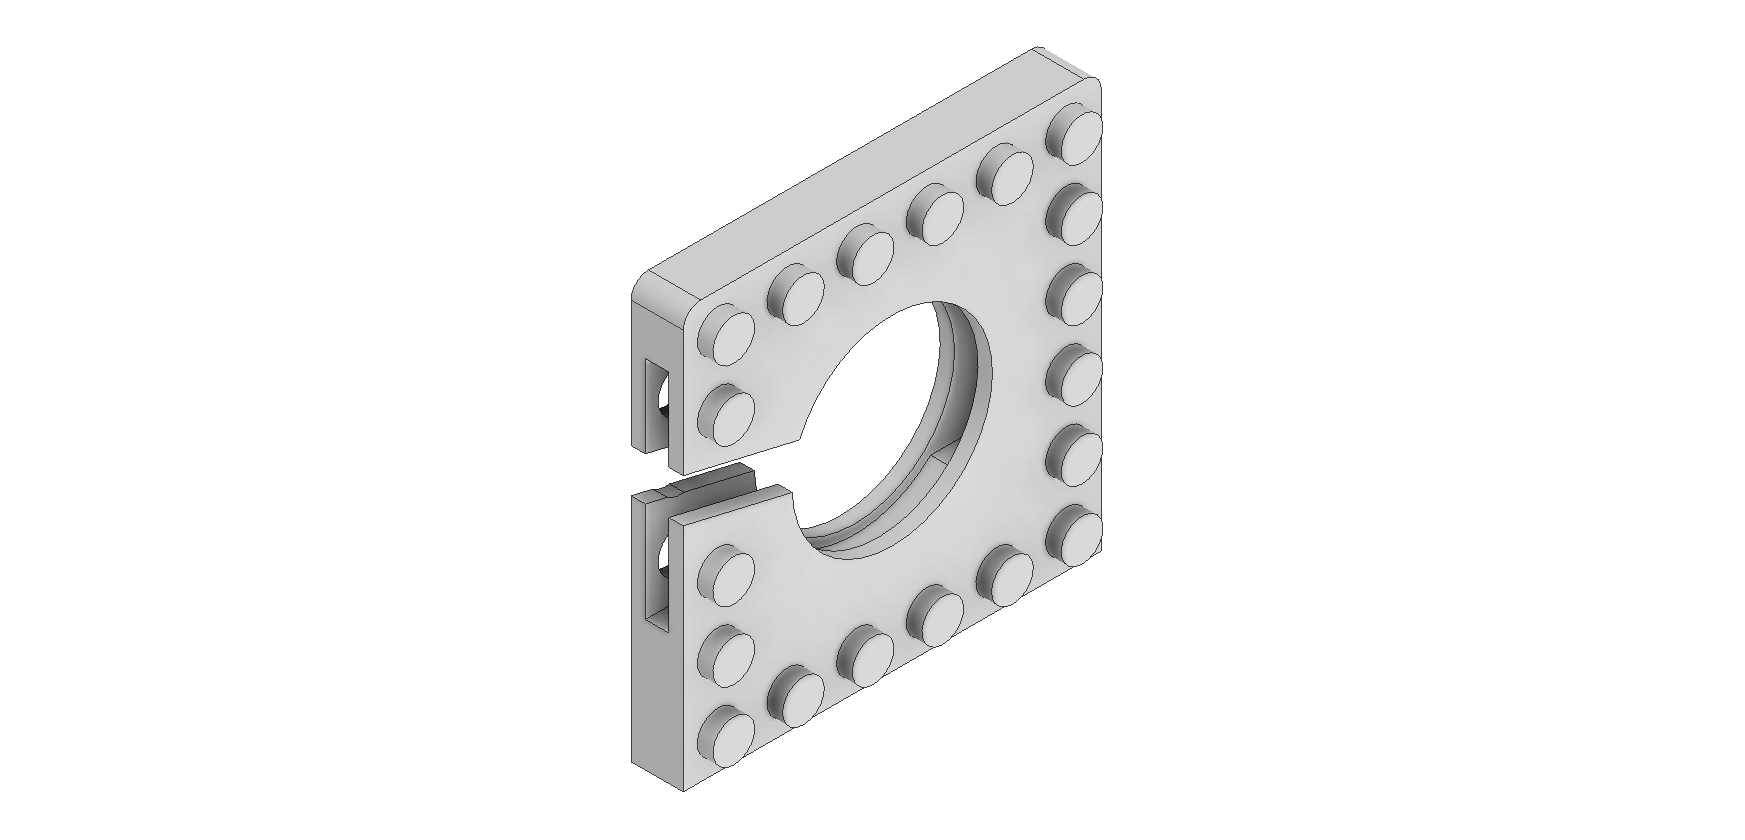
\includegraphics[width=\textwidth]{figures/ch3/fig3_19_Diffuser_Mount.png}
    \caption{擴散片座 (Diffuser\_Mount)}
    \label{fig:part_diffuser_mount}
\end{figure}

相機轉接座 (Camera\_Mount)：作為 Raspberry Pi Camera Module 2 與光學系統的連接橋樑。其內部設計有精確的 PCB 固定柱，並預留了空間供相機本體與排線走線使用，能確保影像感測器（CMOS）平面與顯微鏡的成像光軸維持絕對垂直，避免產生像場彎曲或不均勻散焦。此外，由於系統從上到下皆透過標準化的樂高積木進行定位與固定，這確保了整個光學系統在垂直軸向上的高度同軸性。
\begin{figure}[H]
    \centering
    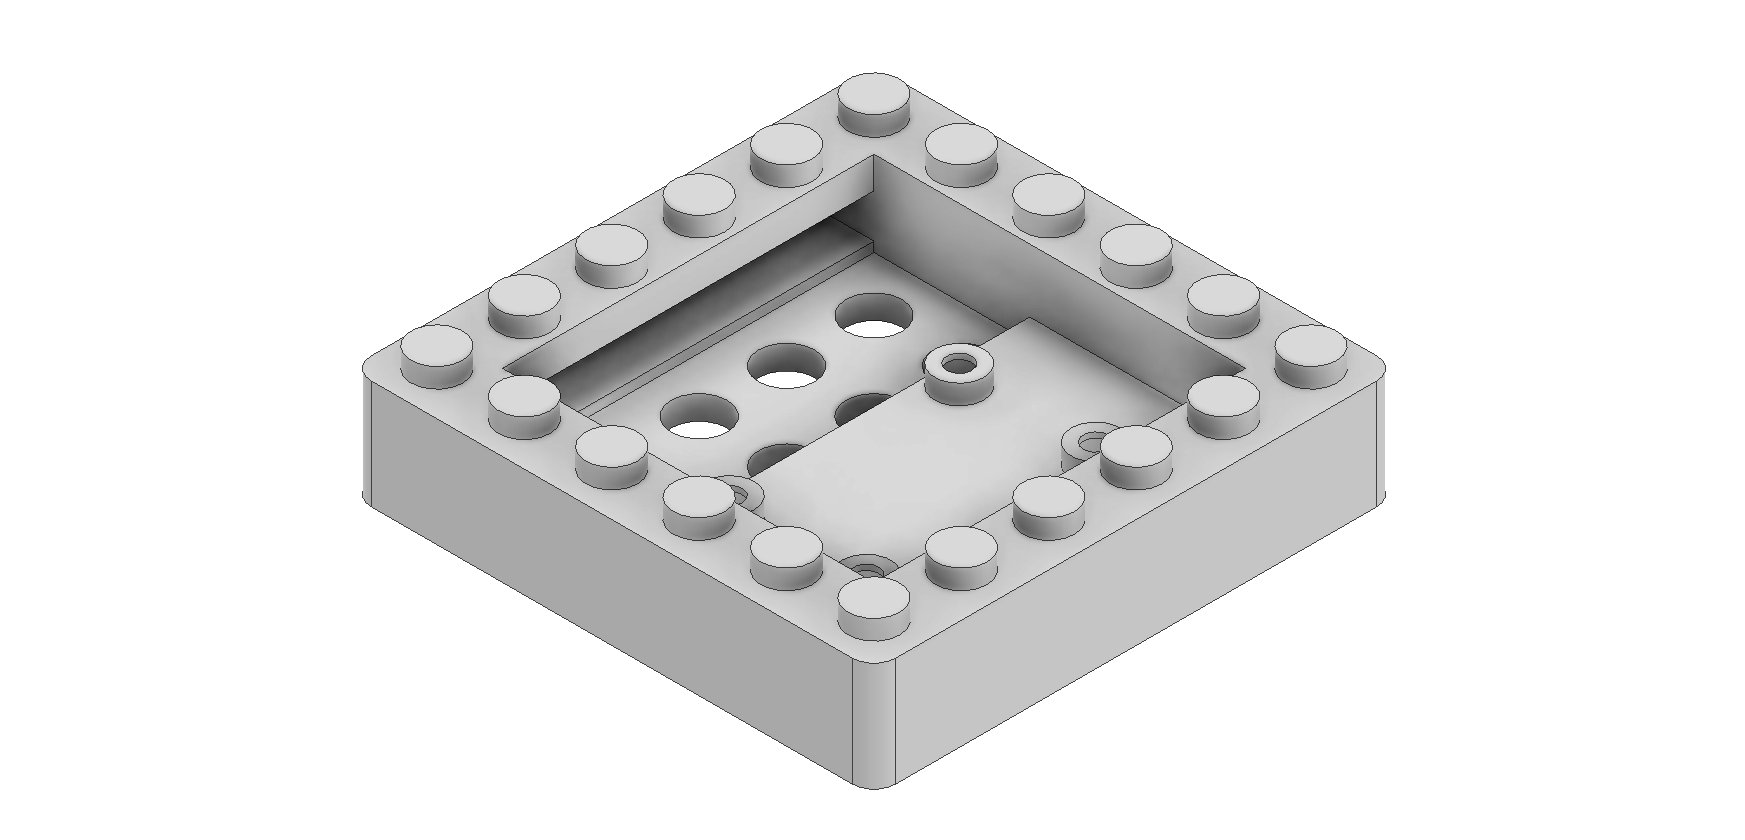
\includegraphics[width=\textwidth]{figures/ch3/fig3_20_Camera_Mount.png}
    \caption{相機轉接座 (Camera\_Mount)}
    \label{fig:part_camera_mount}
\end{figure}
